\documentclass[a4paper]{article}
\usepackage[spanish]{babel}
\usepackage[utf8]{inputenc}
\usepackage{graphicx}
\usepackage{enumerate}
\usepackage{listings}
\usepackage{color}
\usepackage{indentfirst}
\usepackage{fancyhdr}
\usepackage{latexsym}
\usepackage[colorlinks=true, linkcolor=black]{hyperref}
%\usepackage{makeidx}
%\usepackage{float}
\usepackage{wrapfig}
\usepackage{calc}
\usepackage{amsmath, amsthm, amssymb}
\usepackage{amsfonts}
%\lstset{language=C}
\definecolor{gray}{gray}{0.5}
\definecolor{light-gray}{gray}{0.95}
\definecolor{orange}{rgb}{1,0.5,0}

\usepackage{fancyhdr}
\pagestyle{fancy}

%\renewcommand{\chaptermark}[1]{\markboth{#1}{}}
\renewcommand{\sectionmark}[1]{\markright{\thesection\ - #1}}

\fancyhf{}

\fancyhead[LO]{Sección \rightmark} % \thesection\ 
\fancyfoot[LO]{\small{Yanet Giuseppin, Laura Muiño, Javier San Miguel, Axel Straminsky}}
\fancyfoot[RO]{\thepage}
\renewcommand{\headrulewidth}{0.5pt}
\renewcommand{\footrulewidth}{0.5pt}
\setlength{\hoffset}{-0.8in}
\setlength{\textwidth}{16cm}
%\setlength{\hoffset}{-1.1cm}
%\setlength{\textwidth}{16cm}
\setlength{\headsep}{0.5cm}
\setlength{\textheight}{25cm}
\setlength{\voffset}{-0.7in}
\setlength{\headwidth}{\textwidth}
\setlength{\headheight}{13.1pt}

\renewcommand{\baselinestretch}{1.1}  % line spacing


% \setcounter{secnumdepth}{2}
\usepackage{underscore}
\usepackage{caratula}
\usepackage{url}
\usepackage{float}
\usepackage{algorithm}
\usepackage[noend]{algpseudocode}





\newcommand{\cod}[1]{{\tt #1}}
\newcommand{\negro}[1]{{\bf #1}}
\newcommand{\ital}[1]{{\em #1}}
\newcommand{\may}[1]{{\sc #1}}
\newcommand{\tab}{\hspace*{2em}}

\hypersetup{
 pdfstartview= {FitH \hypercalcbp{\paperheight-\topmargin-1in-\headheight}},
 pdfauthor={Grupo},
 pdfsubject={Dise\~{n}o}
}

\lstdefinestyle{customc}{
  backgroundcolor=\color{light-gray},
  belowcaptionskip=1\baselineskip,
  breaklines=true,
  numbers=left,
  xleftmargin=\parindent,
  language=C,
  showstringspaces=false,
  basicstyle=\footnotesize\ttfamily,
  keywordstyle=\bfseries\color{blue},
  commentstyle=\itshape\color{gray},
  identifierstyle=\color{black},
  stringstyle=\color{orange},
}

\lstdefinestyle{customasm}{
  backgroundcolor=\color{light-gray},
  belowcaptionskip=1\baselineskip,
  numbers=left,
  xleftmargin=\parindent,
  language=[x86masm]Assembler,
  keywordstyle=\bfseries\color{blue},
  basicstyle=\footnotesize\ttfamily,
  commentstyle=\itshape\color{gray},
}

\lstset{escapechar=@}


\begin{document}

\thispagestyle{empty}
\materia{Métodos Numéricos}
\submateria{Segundo Cuatrimestre de 2015}
\titulo{Trabajo Práctico I}
%\subtitulo{Scheduling}
\integrante{Yanet Giuseppin}{184/11}{yanetagiu@yahoo.com}
\integrante{Laura Muiño}{399/11}{mmuino@dc.uba.ar}
\integrante{Javier San Miguel}{786/10}{javiersm00@fmail.com}
\integrante{Axel Straminsky}{769/11}{axelstraminsky@gmail.com}

\makeatletter

\maketitle
\newpage

\thispagestyle{empty}
\vfill

\thispagestyle{empty}
\vspace{3cm}
\tableofcontents
\newpage

\newenvironment{myindentpar}[1]
{\begin{list}{1}
         {\setlength{\leftmargin}{#1}}
         \item[]
}
{\end{list} }

%\normalsize
\newpage

% -------------------------------------------------------
% Breve explicacion de la base teorica que fundamenta los metodos involucrados en el trabajo, junto con los metodos mismos.  
% -------------------------------------------------------
\section{Introducción Teórica}

\subsection{El Problema y su representación}
Queremos medir temperaturas de un horno industrial cilíndrico utilizado para fundir metales. Dicho horno tiene una pared interior y una exterior, cuyas temperaturas (la de las paredes) son conocidas en determinados puntos. Sabemos que la pared exterior tiene un límite de temperatura máxima, y nuestro objetivo es determinar si dicha temperatura máxima es alcanzada o no. Para ello, buscamos los puntos en el horno cuya temperatura alcance los 500 grados celcius.  Si esta temperatura es cercana al borde exterior se corre peligro por parte de los trabajadores de una hipotética fábrica que utilice dicho horno.


\begin{wrapfigure}{r}{0.5\textwidth}
  \vspace{-20pt}
  \begin{center}
    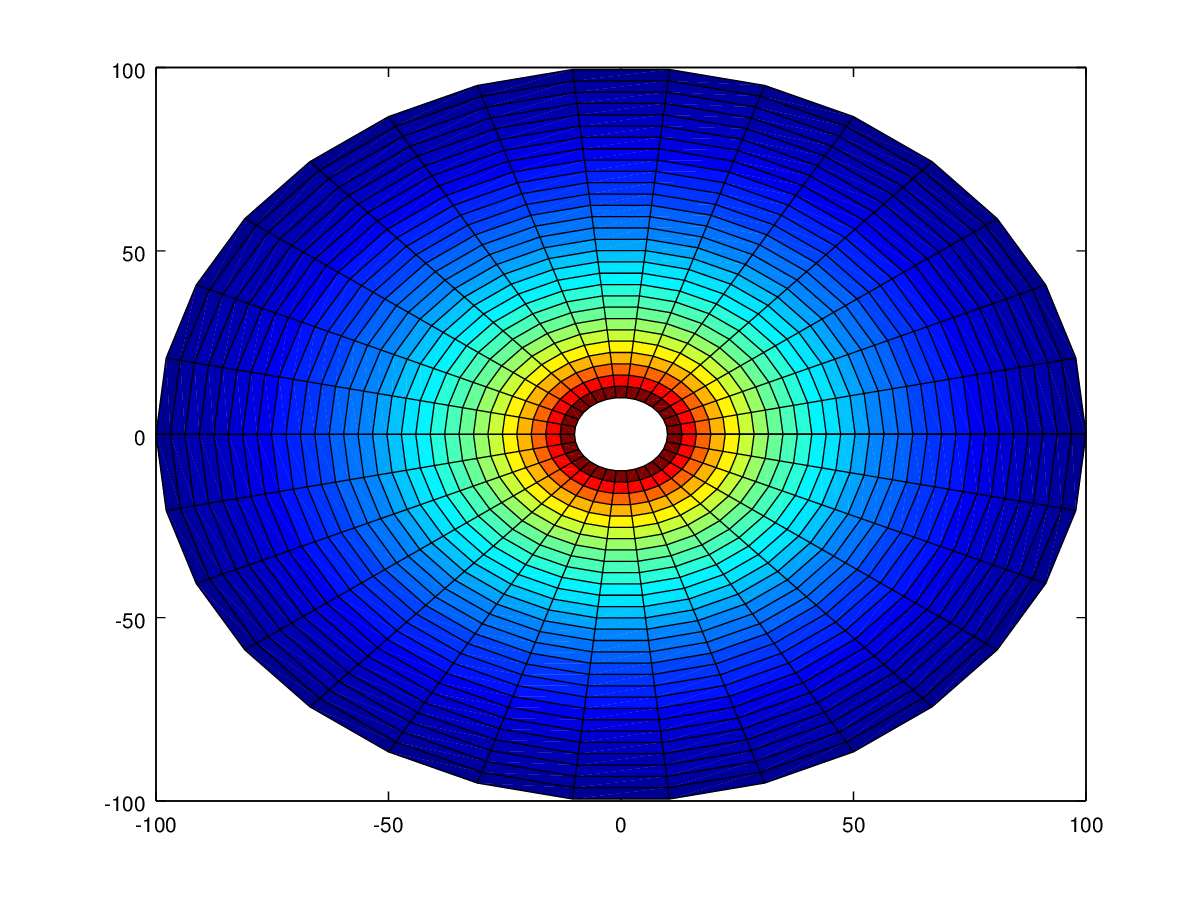
\includegraphics[scale= 0.4]{../hornoEjemplo.png}
  \end{center}
  \vspace{-20pt}
  \caption{Temperatura de un horno.}
  \vspace{-10pt}
  \label{fig:corteHorno}
\end{wrapfigure}


El problema se reduce a determinar dónde se encuentra la isoterma 500 en un círculo, como el que se ve en la figura, que representa un corte del horno. Las pared externa del horno es la circunferencia, y la pared interna es la circunferencia del circulo interno.



\subsection{Solucionando el problema}

Usando las herramientas aprendidas en la materia (sistemas de ecuaciones lineales, y sus métodos de solución, como Eliminación Gaussiana o factorización LU) queremos representar las temperaturas en distintos puntos del horno como incógnitas de un sistema lineal de ecuaciones que resolveremos.
 Para esto vamos a discretizar el espacio para tener finitas incógnitas, y vamos a usar ecuaciones de calor y la información de las temperaturas en finitos puntos de las paredes y así armar la matriz con los coeficientes del sistema.

 %explicar la discretizacion

 % explicar las ecuaciones de calor




A continuación hay una breve introducción a los algoritmos conocidos y teoría que aplicamos y usamos en el trabajo.

\subsubsection{Eliminación Gaussiana}
Dada una matriz A $\in R^{nxn}$ queremos resolver el sistema $Ax = b$. El algoritmo de Eliminación Gaussiana se usa para simplificar el sistema de ecuaciones ya que produce una matriz triangular superior equivalente a la original. Esto facilita el despeje de las incógnitas con el uso de otro algoritmo llamado Backward Substitution. Las tres operaciones principales que se llevan a cabo son, suma entre filas, multiplicación de una fila por un coeficiente distinto de cero e intercambio de filas. Dichas operaciones mantienen la equivalencia.

\subsubsection{Backward Substitution}
El método Backward Substitution consiste en la obtención de los valores de las incógnitas a partir de la matriz triangulada. El método recorre cada fila de esta matriz en orden decreciente en filas. Con lo que el despeje de las incógnitas simplemente consiste en despejar el valor de la diagonal respecto al resto de los valores ya obtenidos en iteraciones anteriores.

\subsubsection{Factorización LU}
El algoritmo de Factorización LU surge ante el problema que se presenta cuando queremos resolver un sistema de ecuaciones similar a uno anteriormente resuelto. Dado el sistema de ecuaciones $Ax = b$, una vez obtenida la matriz triangulada, no queda registro alguno de las operaciones realizadas. Si estas fueran guardadas de alguna manera, podríamos reflejarlas en $b^{*}$  para cada nuevo sistema $Ax = b^{*}$. Repetir E.G. tendría un costo adicional de $O(n^{3})$, sin embargo con la factorización LU este costo solo se tiene una sola vez.


\subsection{Bibliografía}

\begin{itemize}
\item Burden y J.D.Faires, Análisis numérico, International Thomson Editors
\end{itemize}
\newpage
% ------------------------------------------------------
% Análisis de los coef. de la fórmula temperatura.
% -------------------------------------------------------
\section{Desarrollo}

\subsection{Planteo del Sistema}



\begin{wrapfigure}{r}{0.5\textwidth}
  \vspace{-20pt}
  \begin{center}
    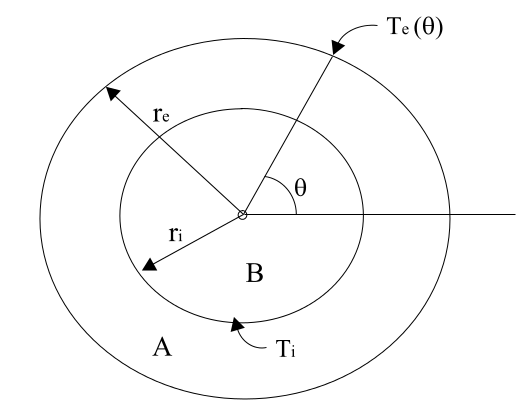
\includegraphics[scale= 0.4]{../Horno.png}
  \end{center}
  \vspace{-20pt}
  \caption{Corte del horno}
  \vspace{-10pt}
  \label{fig:corteHorno}
\end{wrapfigure}


Una instancia del problema equivale a un corte del horno como se ilustra en la figura ~\ref{fig:corteHorno}. Dado que la medición de temperatura en el horno puede realizarse en infinitos puntos, discretizamos el problema fijando la ubicación de los mismos de la siguiente manera; Dividimos el horno en \textbf{\textit{n}} cantidad de ángulos de tamaño $\Delta_{\theta}$ y en \textbf{\textit{m + 1}} cantidad de radios, de tamaño $\Delta_{r}$. Analizaremos las temperaturas en los puntos donde se unen las divisiones entre ángulos y radios. Recordemos que los puntos de la pared interna y externa son dato.\\
\\

La temperatura en un punto $t_{(j,k)}$, con $j \in [0, m]$ y $k \in [0, n)$ estará determinado por la ecuación de Laplace descripta a continuación:


$$ \frac{\partial^{2}T(r,\theta)}{\partial r^{2}} + \frac{1}{r} \frac{\partial T(r,\theta)}{\partial r} + \frac{1}{r^{2}} \frac{\partial^{2}T(r,\theta)}{\partial \theta^{2}} = 0$$\\

Sin embargo utilizaremos una aproximación de esta función que depende de los cuatro puntos que rodean a $t_{(j,k)}$:


$$ \frac{t_{(j-1,k)} - 2t_{(j,k)} + t_{(j+1,k)}}{\Delta_{r} ^{2}} + \frac{1}{r} \frac{t_{(j,k)} - t_{(j-1,k)}}{\Delta_{r}} + \frac{1}{r^{2}} \frac{t_{(j,k-1)} - 2t_{(j,k)} + t_{(j,k+1)}}{\Delta_{\theta} ^{2}} = 0$$

Despejamos las incógnitas $t_{(j,k)}$, $t_{(j+1,k)}$, $t_{(j-1,k)}$, $t_{(j,k+1)}$ y $t_{(j,k-1)}$ para obtener una ecuación (un sistema de ecuaciones) que dependa de ellas. Resulta la siguiente fórmula:



$$  t_{(j,k)} (-\frac{2}{\Delta^2_r}+\frac{1}{r \Delta_r}-\frac{2}{r^2 \Delta^2_\theta}) + t_{(j+1,k)} (\frac{1}{\Delta^2_r}) + t_{(j-1,k)} (\frac{1}{\Delta^2_r}-\frac{1}{r \Delta_r}) + t_{(j,k+1)} (\frac{1}{r^2 \Delta^2_\theta}) + t_{(j,k-1)} (\frac{1}{r^2 \Delta^2_\theta}) = 0$$ \\


Una vez planteadas estas ecuaciones para cada $ t_{(j,k)} $, resolvemos que el sistema $Ax = b$ estará formado por $n*m$ ecuaciones con la misma cantidad de incógnitas. El valor lo justificamos debido a la cantidad de combinaciones entre los índices j y k (cantidad de ángulos por cantidad de radios). Otra forma de razonar este resultado es pensando que en cada anillo generado por la partición del horno en \textbf{\textit{m + 1}} radios, habrá \textbf{\textit{n}} incógnitas generadas a su vez por la particion en ángulos. \\
Esta cantidad incluye los valores $t_{(0,k)}$ y $t_{(n-1,k)}$ (los valores de temperatura en la pared interior y exterior respectivamente), por lo que en sus ecuaciones habrá un único coeficiente con valor 1 en la posición que corresponde a estas incógnitas y su valor b será el que se pase por parámetro. Para el resto de los $t_{(j,k)}$ los coeficientes corresponderan a los coeficientes descriptos en la ecuación de arriba, y su b será cero, también respetando dicha ecuación.

\subsection{Orden de los coeficientes}

Para conseguir una matriz banda, decidimos ordenar los coeficientes de manera creciente respecto al índice de los radios \textbf{\textit{j}} y luego respecto a \textbf{\textit{k}} el índice de los ángulos. Para ilustrar el orden impuesto, exponemos el siguiente ejemplo:

Sea $\Delta_{r} = \Delta{\theta} = 1$, $\textbf{\textit{m + 1}} = \textbf{\textit{n}} = 3$ el orden resultante será 

$$ t_{(0,0)} t_{(0,1)} t_{(0,2)} ...... t_{(2,0)} t_{(2,1)} t_{(2,2)} $$

Y la matriz de coeficientes queda como la siguiente:\\



\begin{figure}[h]
  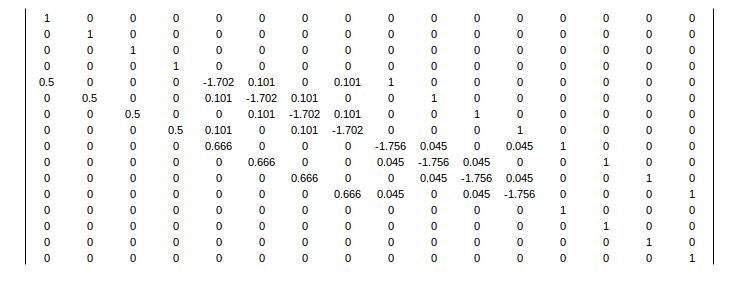
\includegraphics[width=\textwidth]{imagenes/matrizEjemplo.png}
  %\caption{Matriz de ejemplo}
  %\label{fig:corteHorno}
\end{figure}



\begin{figure}[h]
  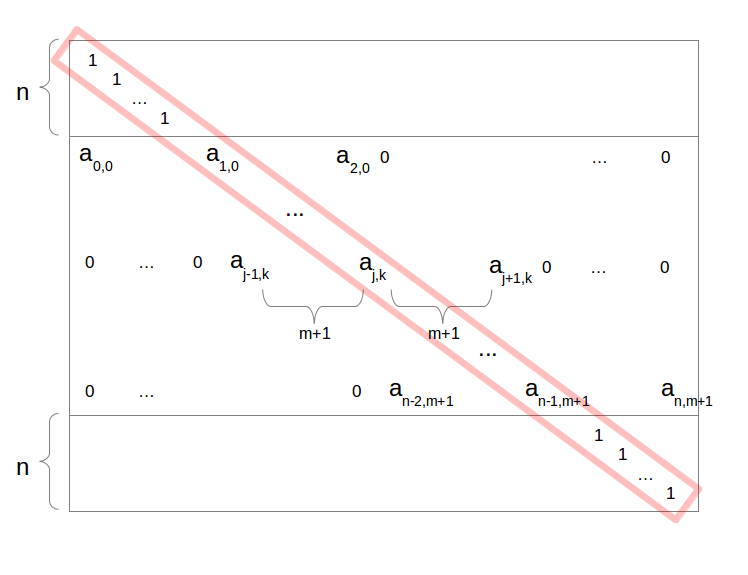
\includegraphics[scale=0.4]{imagenes/figura1.png}
  \caption{La figura}
  \label{fig:corteHorno}
\end{figure}

%---------------------------------------------------------------------

\subsection{Análisis de Coeficientes}
A partir de las aproximaciones de las derivadas parciales de la función $T$ distribuimos los términos para conocer los coeficientes asociados a cada punto del cual depende el valor de la temperatura que queremos conocer para un $j,k$ dado. Se debe cumplir la siguiente ecuación: \\
$$t_{(j-1, k)} (\frac{1}{\Delta^2_r}-\frac{1}{r \Delta_r}) +
t_{(j, k)} (-\frac{2}{\Delta^2_r}+\frac{1}{r \Delta_r}-\frac{2}{r^2 \Delta^2_\theta}) + 
t_{(j+1, k)} (\frac{1}{\Delta^2_r}) + 
t_{(j, k-1)} (\frac{1}{r^2 \Delta^2_\theta}) +
t_{(j, k+1)} (\frac{1}{r^2 \Delta^2_\theta}) = 0 $$ \\

Analizamos los casos en que los coeficientes obtenidos a partir de la discretización de las derivadas parciales asociados a cada punto se anulan, es decir, para que $r, \Delta_r,$ y $\Delta_\theta$ el coeficiente se anula. \\
Para el coeficiente asociado a $t_{(j-1, k)}$, $r$ debe valer $\Delta_r$. Como $r_j = (j \Delta_r) + r_i$ esto se cumple si $j$ vale 1 y $r_i$ vale cero, o $j$ vale cero y $r_i$ vale $\Delta_r$. Para el primer caso, significa que el horno no tiene radio interno, mientras que la segunda no puede suceder puesto que la ecuación la cumplen solo las temperaturas entre el radio interno y el externo (no incluidos) y si $j$ vale cero, indica que es el radio interno.
Para los coeficientes de $t_{(j+1, k)}$, $t_{(j, k-1)}$ y $t_{(j, k+1)}$, los coeficientes nunca se anulan. \\
Por último, para el coeficiente asociado a $t_{(j, k)}$, desarrollamos las sumas e igualamos a cero. \\
$$\frac{-2r^2 \Delta^2_\theta + r \Delta_r \Delta^2_\theta - 2 \Delta^2_r}{\Delta^2_r r^2 \Delta^2_\theta} = 0$$\\
El término inferior nunca se anula, por lo que debería anularse el término superior. Observamos que corresponde a una función cuadrática siendo $r$ la variable. Desarrollamos la fórmula de Bhaskara obteniendo: \\
$$r = \frac{\Delta_r}{4} \pm \frac{\sqrt{\Delta^2_r \Delta^4_\theta - 16 \Delta_\theta \Delta^2_r}}{4 \Delta^2_\theta}$$ \\
El análisis se vuelve muy complicado, pero nos valemos de saber que para que el planteo tenga sentido, $r$ debe ser mayor o igual que $\Delta_r$.
El segundo miembro es siempre positivo, por lo que si se le resta algo positivo a $\frac{\Delta_r}{4}$, seria aún menor, por lo tanto solo queda analizar el caso en que se suman los términos. Para que se cumpla la condición $\Delta_r \leq r$, queremos encontrar los $\Delta_r$ y $\Delta_\theta$ tal que: \\
$$\frac{3 \Delta_r}{4}  \leq \frac{\sqrt{\Delta^2_r \Delta^4_\theta - 16 \Delta_\theta \Delta^2_r}}{d \Delta^2_\theta} $$ \\
Para este fin, utilizamos la página web $www.wolframalpha.com$ para encontrar las soluciones al problema, las cuales indican que si $\Delta_r$ es positivo, $\Delta_\theta$ debe ser menor a cero y viceversa. Por lo tanto, el coeficiente se anula solamente para valores que no tienen sentido dentro del problema. \\
%http://www.wolframalpha.com/input/?i=sqrt%28x^2+y^4+-+16+x^2+y%29+%2F+%284*y^2%29+%3E%3D+3x%2F4
Con este análisis, concluimos que los coeficientes obtenidos de la ecuación no se anulan en los casos en que el problema planteado tiene sentido.

%---------------------------------------------------------------------

\subsection{Análisis de Pivoteo}

Para justificar que en la matriz banda no se produce pivoteo al aplicarse el algoritmo de Eliminación Gaussiana, procedemos a demostrar que la matriz banda es diagonal dominante. Con esto llegamos a la conclusión de que es no singular. Con esto se tiene  que la matriz tiene factorización LU, con lo cual no se produce pivoteo en la E.G.


%---------------------------------------------------------------------


\subsubsection{A es diagonal dominante}
Queremos ver que A es diagonal dominante, es decir, que se cumple la siguiente inecuación:\\
$$\mid \frac{1}{\Delta^2_r}-\frac{1}{r \Delta_r}\mid +
\mid \frac{1}{\Delta^2_r} \mid + 
\mid \frac{1}{r^2 \Delta^2_\theta} \mid +
\mid \frac{1}{r^2 \Delta^2_\theta} \mid
\leq \mid -\frac{2}{\Delta^2_r}+\frac{1}{r \Delta_r}-\frac{2}{r^2 \Delta^2_\theta} \mid$$  \\
Primero, nos deshacemos de los módulos. El primer término es negativo solo cuando $r < {\Delta_r}$, pero esto no sucede debido a que $r= j \Delta_r + r_i$, con $j$ natural y $r_i$ real positivo. El resto de los términos a la izquierda de la desigualdad tambien son positivos debido a que todas las viariables estan elevadas al cuadrado, por lo tanto es equivalente no tomar módulo para estos términos. \\
Para el término de la derecha, $-\frac{2}{r^2 \Delta^2_\theta}$ siempre es negativo, por lo que para que el término sea positivo, $-\frac{2}{\Delta^2_r}+\frac{1}{r \Delta_r}$ debe de ser necesariamente positivo. Sin embargo, esto solo puede ocurrir cuando $r < \frac{\Delta_r}{2}$, por lo que siempre resulta negativo por el argumento anterior. De este modo, si multiplicamos este término por -1, obtenemos un número positivo. La inecuación resultante es: \\ 
$$ \frac{1}{\Delta^2_r}-\frac{1}{r \Delta_r} +  
\frac{1}{\Delta^2_r} + 
\frac{1}{r^2 \Delta^2_\theta} +
\frac{1}{r^2 \Delta^2_\theta}
\leq \frac{2}{\Delta^2_r}-\frac{1}{r \Delta_r}+\frac{2}{r^2 \Delta^2_\theta}$$ \\

Sumamos los términos y obtenemos: \\
$$\frac{2}{\Delta^2_r}-\frac{1}{r \Delta_r}+\frac{2}{r^2 \Delta^2_\theta} \leq \frac{2}{\Delta^2_r}-\frac{1}{r \Delta_r}+\frac{2}{r^2 \Delta^2_\theta}$$ \\
Podemos observar que se cumple la inecuación como queríamos demostrar, y en particular, vale la igualdad.


%---------------------------------------------------------------------

\subsubsection{A es no singular}
Dada la matriz A diagonal dominante, veamos que A es no singular.
Por absurdo supongamos que es singular, esto es, $\exists x\neq 0$ tal que $x \in Nu(A)$.
Como el vector es distinto a cero, existe una coordenada que es mayor al resto. Llamémosla $x_{k}$.


Del sistema de ecuaciones Ax, tomemos la ecuación k, que tiene esta forma:                  

$$ a_{(k, 1)} * x_{1} + a_{(k, 2)} * x_{2} +... + a_{(k, n)} * x_{n} = 0 $$\\

Luego despejamos el término k y aplicamos módulo:\\

 $$ \mid a_{(k, k)} * x_{k} \mid  =  \left \arrowvert - \sum_{j=1,j\neq k}^{n}  a_{(k,j)} * x_{j} \right \arrowvert $$

 $$ \mid a_{(k, k)}\mid * \mid x_{k} \mid \leq \sum_{j=1,j\neq k}^{n} \mid a_{(k,j)}\mid * \mid x_{j} \mid $$


 $$ \mid a_{(k, k)}\mid  = \sum_{j=1,j\neq k}^{n} \mid a_{(k,j)}\mid *  \frac{\mid x_{j} \mid}{\mid x_{k} \mid}$$\\

Anteriormente probamos que A es diagonal dominante y que en particular vale la igualdad. Como cada elemento de la sumatoria (que vale exactamente $a_{(k, k)}$) es multiplicado por $\frac{\mid x_{j} \mid}{\mid x_{k} \mid}$ $\leq 1$, disminuyen su valor, con lo que la sumatoria se reduce y resulta:\\

$$\mid a_{(k,k)} \mid < \sum_{j=1, j\neq k}^{n}\mid a_{(k,j)} \mid $$\\

Lo que es absurdo, pues A era diagonal dominante. El absurdo provino de suponer que A es singular. Luego vale que A es no singular.

%---------------------------------------------------------------------

\subsubsection{A tiene factorización LU}

%---------------------------------------------------------------------

\subsection{Problemas que nos encontramos durante el desarrollo}

\begin{itemize}
\item Nos encontramos con problemas a la hora de cargar la matriz A de coeficientes. Lo solucionamos realizando ejemplos de un tamaño razonable en papel, y chequeando a mano que las distintas filas estuvieran bien cargadas.

\item Problemas de precisión numérica. Inicialmente los resultados de los\ tests diferían con los resultados de la cátedra. Debido a los problemas inherentes a la aritmética de punto flotante, comenzamos experimentando con distintas maneras de realizar la sumatoria (ordenando los números de mayor a menor y de menor a mayor), ya que pensabamos que estabamos arrastrando un error. Descubrimos que las distintas maneras de realizar las sumatorias diferían en menos de $0,00001$, por lo que concluímos que no estabamos arrastrando errores en las cuentas. Finalmente descubrimos que el error estaba en que la variable $m$ en realidad era $m+1$, y no teníamos eso en cuenta a la hora de calcular $\Delta r$.

\end{itemize}
\newpage

\section{Experimentación}

Queremos ver empíricamente que las complejidades de los algoritmos es la cota teórica demostrada en la sección de desarrollo. Para esto se diseñaron una serie de tests que fueron generados con el programa \textit{generatetest.py}. En estos, el ángulo fue fijado en $10$, y el radio ($m$) fue variando entre $5$ y $80$.
Cada archivo de test tiene $40$ instancias en las que los valores de las paredes internas y externas son aleatorios y varían en un determinado valor respecto de los valores adyacentes.

Como lo que nos interesa medir es el tiempo de ejecución y éste depende del tamaño de la matriz, con variar $n$ o $m$ ya basta para ver como aumentan los tiempos en función del tamaño.

Los tests fueron corridos en una CPU Intel I5-760 de 2.80 Ghz.

Medimos para cada test el tiempo total en resolver las 40 instancias, para evitar que la presencia de outliers influyera de manera significativa en los tiempos de ejecución. No tuvimos en cuenta los tiempos de carga de las matrices y vectores.

Para el siguiente gráfico lo que hicimos fue dividir el tiempo de ejecución ($O(m^{3})$) por $m^{2}$, para de esta manera obtener el gráfico de una recta y probar efectivamente que el tiempo de ejecución real del algoritmo de Eliminación Gaussiana es el dicho anteriormente.

\begin{figure}[h]
  \center
  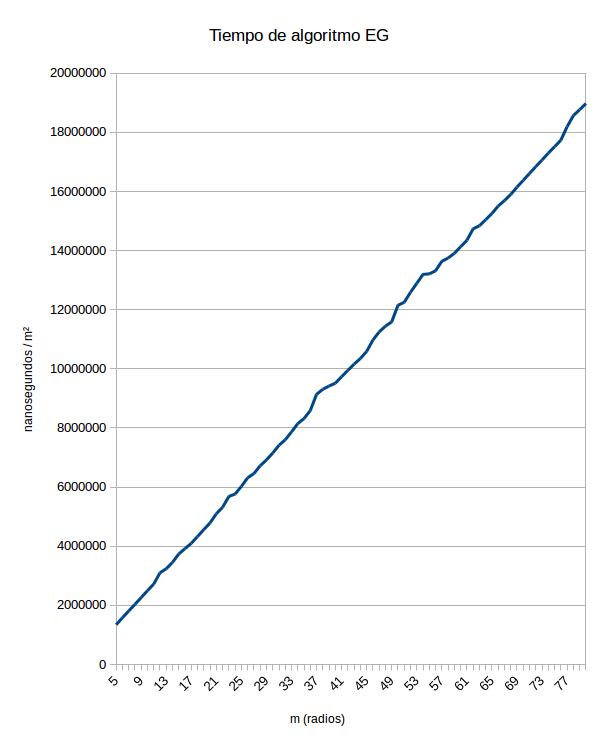
\includegraphics[scale=0.8]{imagenes/tiempoEGdivididoM2.png}
  %\caption{La figura}
  \label{fig:egdivididom2}
\end{figure}

En el gráfico a continuación, lo que hicimos fue considerar 2 casos: contando el tiempo de obtención de las matrices L y U, y sin contarlo. En ambos casos dividimos el tiempo de ejecución por $m$. En el primer caso, al dividir por $m$, el gráfico crece de manera parabólica, ya que el tiempo que tarda el algoritmo en obtener las matrices L y U es $O(m^{3})$. Por lo tanto, al dividir por m, el tiempo de ejecución debería crecer de forma cuadrática, lo cual se puede observar en el gráfico. 


\begin{figure}[h]
  \center
  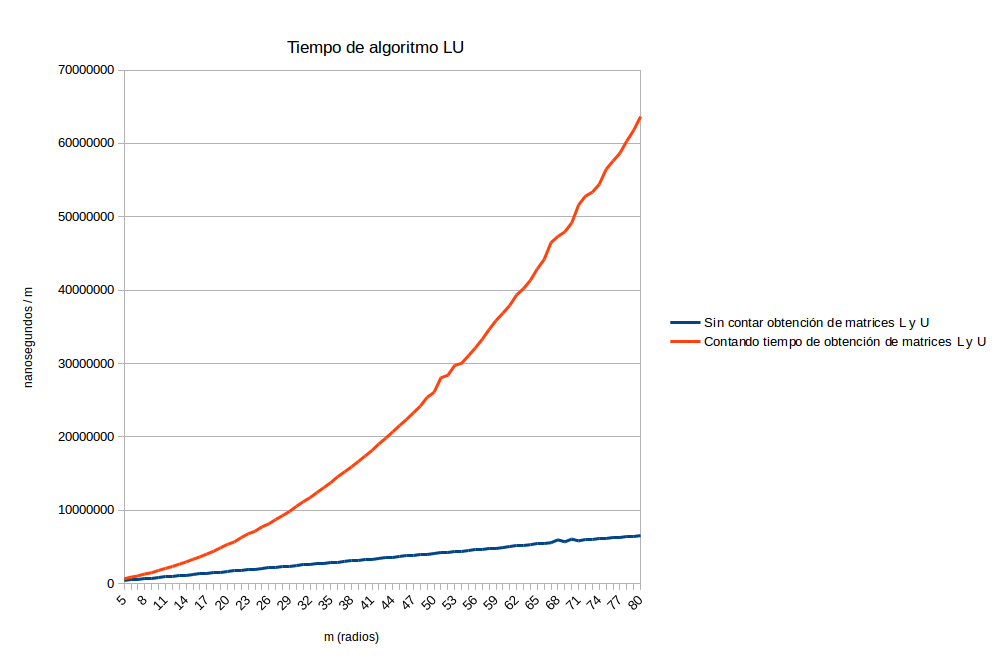
\includegraphics[scale=0.6]{imagenes/tiempoLUdivididoM.png}
  %\caption{La figura}
  \label{fig:ludivididom}
\end{figure}


En el segundo caso no se tuvo en cuenta el tiempo de obtención de las matrices L y U, por lo tanto el tiempo de ejecución del algoritmo es $O(m^{2})$, y al dividir todo por $m$, obtenemos una recta, como se puede observar. \\


Por último vamos a comparar directamente el tiempo de ejecución de la eliminación gaussiana contra el tiempo de ejecución de LU (contando el tiempo de obtención de la matriz LU). En este caso los tiempos de ejecución no fueron divididos por $m$ ya que solamente queríamos poder comparar a grandes rasgos las diferencias entre los tiempos de ejecución de ambos algoritmos. Por más que ambos algoritmos son $O(m^{3})$, se puede observar que la eliminación gaussiana toma considerablemente más tiempo, lo cual nos confirma empíricamente la importancia de guardarnos las matrices L y U a la hora de resolver un sistema de ecuaciones.

\newpage

\begin{figure}[h]
  \center
  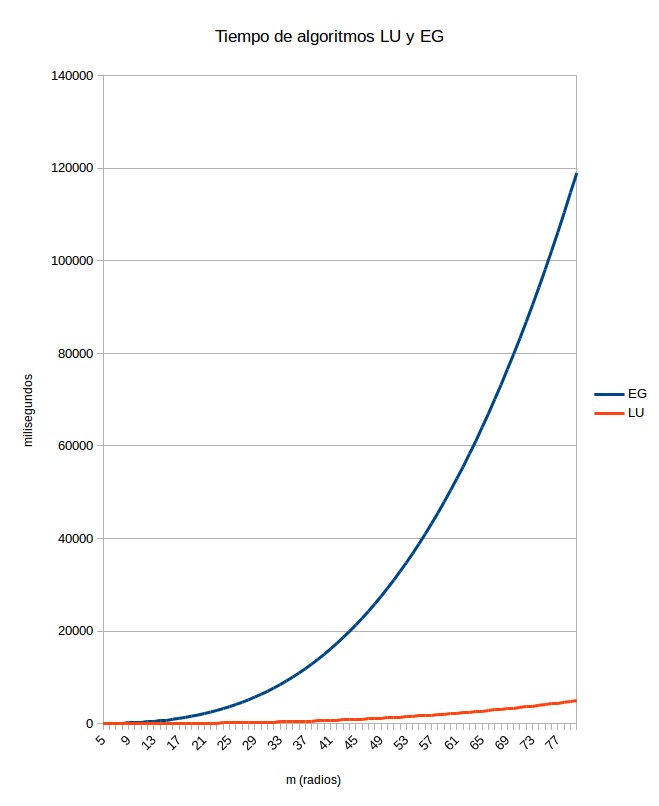
\includegraphics[scale=0.8]{imagenes/tiempoLUyEGsinDividir.png}
  %\caption{La figura}
  \label{fig:luyeg}
\end{figure}


\newpage

\section{Resultados}

\subsection{Experimentos Planteados}



\begin{wrapfigure}{r}{0.5\textwidth}
  \vspace{-20pt}
  \begin{center}
    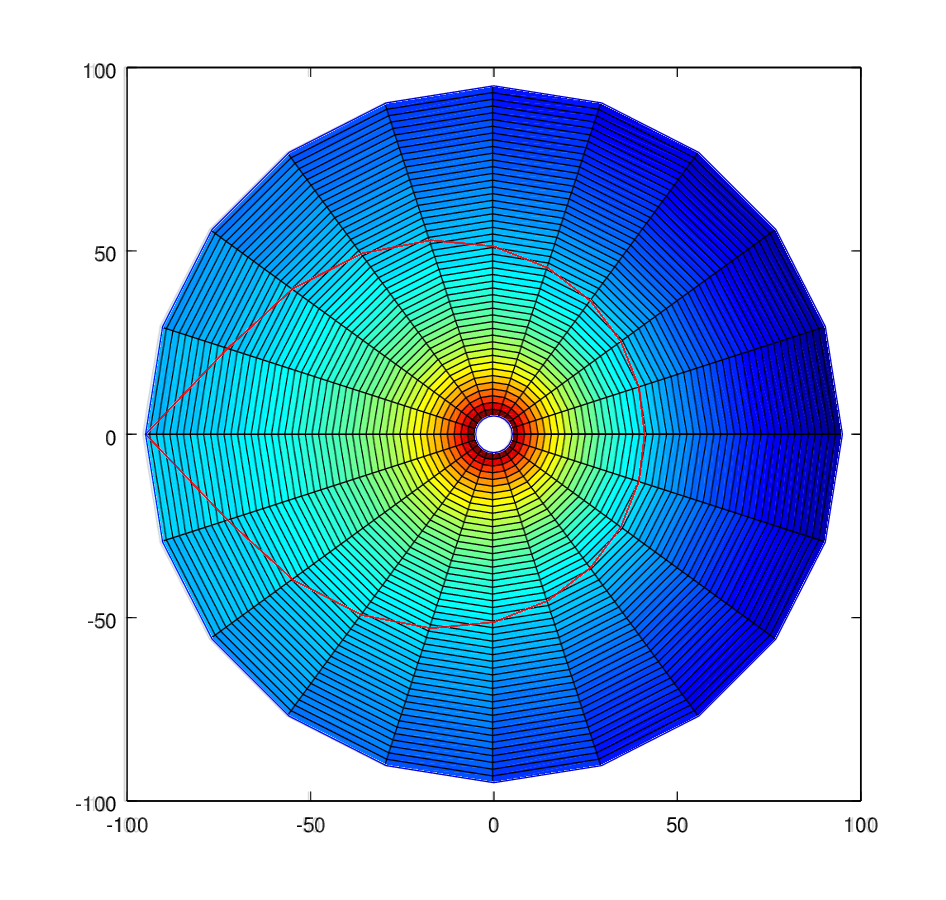
\includegraphics[scale= 0.4]{imagenes/hornoColorSubeBajaConIsoterma.png}
  \end{center}
  \vspace{-20pt}
  \caption{Experimento 1}
  \vspace{-10pt}
  \label{fig:Exp1}
\end{wrapfigure}

El primer experimento planteado consistió en generar una instancia del problema donde los valores de las temperaturas externas varíen gradualmente desde 0 hasta la isoterma pedida. Para esto generamos una instancia con $n=20$, donde para el primer ángulo, la temperatura de la pared externa, vale $0$, y luego aumenta en sentido anti-horario en 50. Al llegar a la mitad de la circunferencia, llega a valer 500 y luego decrece nuevamente. La idea de este experimento consistió en ver la variación de la isoterma y además aprovechar esta variación para estudiar para cada ángulo, la variación de la temperatura para cada punto obtenido.
\\
\begin{wrapfigure}{r}{0.5\textwidth}
  \vspace{-20pt}
  \begin{center}
    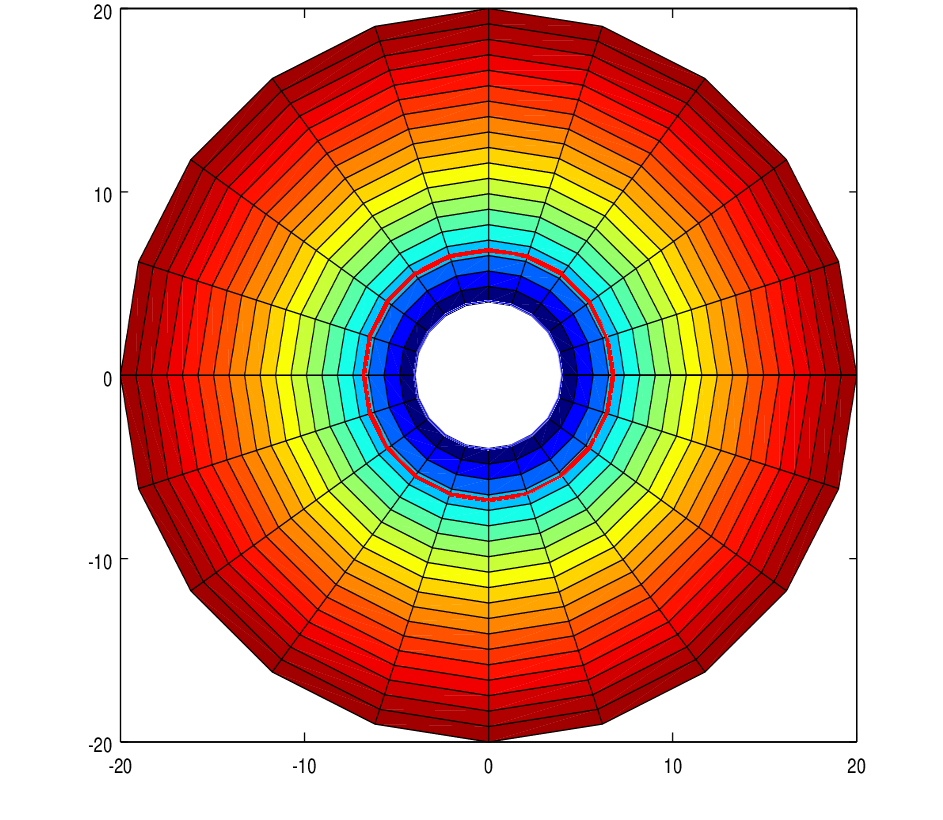
\includegraphics[scale= 0.4]{imagenes/hornoInvertidColoroConIso.png}
  \end{center}
  \vspace{-20pt}
  \caption{Experimento 2}
  \vspace{-10pt}
  \label{fig:Exp1}
\end{wrapfigure}

El segundo experimento planteado consistió en generar una instancia del problema donde los valores de las temperaturas se encuentren invertidas, es decir, las temperaturas internas son menores que las externas. Para esto generamos una instancia con $n=20$, con las paredes internas valiendo 0 y las externas valiendo 1500. La idea de este experimento consistió en ver si en la ecuación planteada seguía teniendo sentido y si nos topabamos con una solución razonable del sistema o si nos encontraríamos con algún error.
\\
%Para ambas figuras se marcaron los valores de la isoterma encontrada
\begin{wrapfigure}{l}{0.5\textwidth}
  \vspace{-20pt}
  \begin{center}
    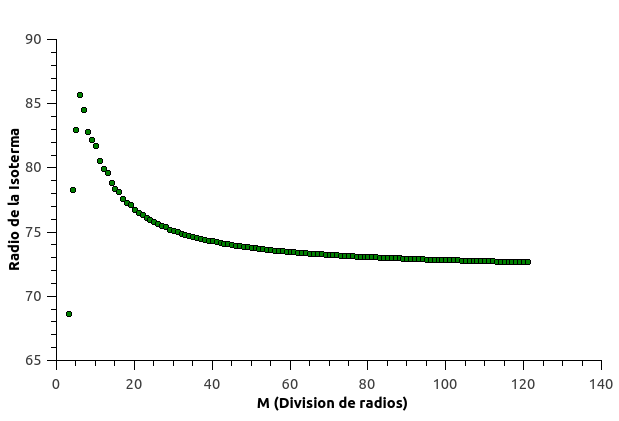
\includegraphics[scale= 0.4]{imagenes/graphDiscretizacionv2.png}
  \end{center}
  \vspace{-20pt}
  \caption{Experimento 3}
  \vspace{-10pt}
  \label{fig:Exp3}
\end{wrapfigure}

El tercer experimento planteado consistió en estudiar el impacto de incrementar la discretización de los radios (aumentar el $m$) y ver cómo impacta en la obtención de la isoterma. Se usó una instancia donde los valores internos valen 1500, los externos valen 0 y la diferencia entre el radio interno y el externo es 100. Empezamos tomando $m=3$ y lo aumentamos de a 1 hasta llegar a $m=120$, manteniendo todos los parámetros igual. De este modo, podemos observar cómo impacta la discretización del radio en el valor del radio obtenido de la isoterma.\\
%Una instancia del problema equivale a un corte del horno como se ilustra en la figura ~\ref{fig:Exp1}. Dado que la medición de temperatura en el horno puede realizarse en infinitos puntos, discretizamos el problema fijando la ubicación de los mismos de la siguiente manera; Dividimos el horno en \textbf{\textit{n}} cantidad de ángulos de tamaño $\Delta_{\theta}$ y en \textbf{\textit{m + 1}} cantidad de radios, de tamaño $\Delta_{r}$. Analizaremos las temperaturas en los puntos donde se unen las divisiones entre ángulos y radios. Recordemos que los puntos de la pared interna y externa son dato.\\
%\\
\newpage

\section{Discusión}
En primer lugar, utilizamos el experimento 1 para poder analizar las variacion de la temperatura para cada angulo del horno. Graficamos los resultados obtenidos para cada radio para observar como se comporta la discipacion del calor en función del radio. De este modo, podriamos entender mejor como se comporta la función para sacar conclusiones de como obtener una mejor aproximacion para encontrar la isoterma pedida.

\begin{figure}[h]
  \center
  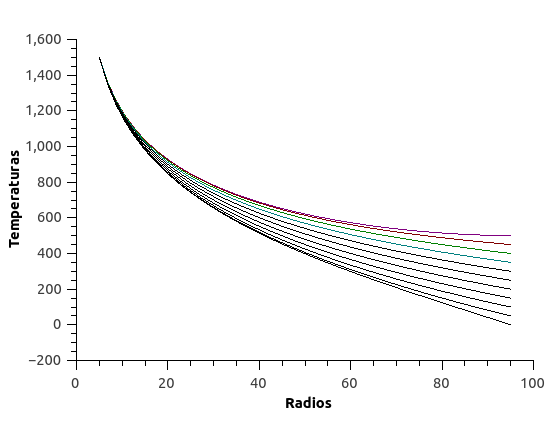
\includegraphics[scale=0.8]{imagenes/avanceTemperaturas.png}
  %\caption{La figura}
  \label{fig:avanceTemps}
\end{figure}

Cada curva corresponde a un angulo del horno y se grafica la temperatura para cada radio. Como se puede ver, se corresponden con la familia de funciones $f(x)= \frac{1}{x}$. De este modo, concluimos que utiliazar una regla de tres simple para aproximar la locación de la isoterma no es una aproximación correcta porque guarda una relación lineal, mientras que los datos revelan una relacion inversa multiplicativa. \\
Sin embargo, no resulta una tarea sencilla encontrar una mejor aproxiamción debido a que si la encontraramos, podriamos resolver el problema inicial sin tener que plantear el sistema de ecuaciones planteado anterior. Por tal razón, analizamos alternativas para encontrar una mejor aproximación. Para eso realizamos el experimento 3, para analizar como aumentando el nivel de discretización para una instancia dada, como impacta en el hallazgo de la isoterma. \\
Nuestra hipótesis era que aumentando el nivel de discretización, se refinara la locación de la isoterma, debido a la forma en que la hallamos es encontrar los dos puntos entre los que se encuentra la isoterma. Aumentando la cantidad de puntos, se disminuye la distancia entre los mismos, por lo que el error introducido por la aproximación también debe disminuir. \\
Nos encontramos con un resultado llamativo, que fue darnos cuenta que los primeros puntos no se correspondian con la funcion graficada, y algunos de los primeros puntos tenian un radio menor al radio al que tiende al función. Esto no debería suceder debido a lo siguiente: 
\newpage

\begin{wrapfigure}{l}{0.5\textwidth}
  \vspace{-20pt}
  \begin{center}
    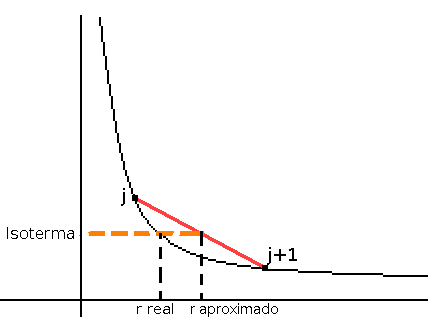
\includegraphics[scale=0.4]{imagenes/aprox.png}
  \end{center}
  \vspace{-20pt}
  \caption{Aproximación lineal contra valor esperado}
  \vspace{-10pt}
  \label{fig:aproximacion}
\end{wrapfigure}

Al utilizar una regla de tres simple, para cada radio obtenido deberíamos obtener un radio ligeramente mayor al radio real de la isoterma, debido a que la función de la discipación del calor tiene una relación inversa multiplicativa.\\
La razón por la que para los primeros valores la función se asemeja a una función lineal, es porque para los primeros casos la isoterma se encuentra entre el radio interno y el siguiente al radio interno. Basamos nuestra aproximación en contar con que el valor de la temperatura hasta el radio $j$ coincide con la función de discipación de calor, y a eso le introducimos un error al aproximar el radio que falta hasta la isoterma. Por lo tanto, si no contamos con valores anteriores al $j$, se cuenta con un error mayor, y la función se asimila más a una lineal que a la que queremos aproximar realmente.\\
Como se ve en la figura \ref{fig:Exp3}, a partir de la instancia en que $m=7$, la función empieza a decrecer y se ve como el valor del radio de la isoterma se estabiliza, debido a que el error se va minimizando por cada nueva división del radio y tiende al valor real del radio de la isoterma.
\newpage

%aca iria apencide
\section{Conclusiones}
Implementamos dos metodos para resolver muchas instancias de sistemas de ecuaciones en los que variaban solamente los términos independientes. \\
Ordenamos las ecuaciones y los coeficientes de las matrices de manera de poder aprovechar que el valor de temperatura de cada punto de la discretización solo depende de otras cuatro temperaturas, haciendo que las matrices tengan muchos ceros. Por esto las implementaciones de los métodos se pudieron simplificar.\\

Analizamos los tiempos de ejecución de ambos, y cómo varían según el tamaño de los sistemas. Vimos después, de manera gráfica, cómo las temperaturas resultantes son las que esperábamos para el interior del horno. Con algunos ejemplos fue suficiente para ver cómo se dispersa el calor.\\

Para la resolución de un problema como este en que las distintas instancias (a medida que transcurre el tiempo) pueden representarse con sistemas de ecuaciones del tipo AX = b donde la matriz A es siempre la misma, concluímos que el mejor método para usar es la factorización LU. Vimos que la complejidad para los dos métodos es la misma si se quiere resolver un sólo sistema, pero la factorización LU reduce la complejidad cuando se quieren resolver sistemas para muchas instancias del problema. Y más aún, para resolver sistemas más grandes la diferencia se amplía mucho.\\

Como conclusión, nos resultó muy interesante la enorme diferencia temporal entre la eliminación Gaussiana y LU. Creimos en un principio que la cantidad de instancias que se iban a poder correr en un tiempo razonable con una implementacion y en la otra no, iban a ser mucho más pequeña. Realmente se ve una diferencia donde una alternativa puede resultar en que un proyecto se vuelva inviable y otra no (por ejemplo, si quisieramos implementar tal sistema en una planta real con sensores en un horno).\\

Tambien analizamos qué sucede cuando cambia el nivel de discretización, cómo afecta esto a los resultados de los sistemas y a los valores de radios de la isoterma, que era en definitiva lo que buscabamos. Mientras más puntos se toman para calcular las temperaturas, más se acercan los resultados obtenidos a los valores de radios reales de la isoterma. La forma en que se estima el valor de la isoterma cuando no se tiene un resultado preciso es importante, ya que nunca se pueden tomar suficientes puntos de discretización siendo el espacio infinito. Hay que tener en cuenta que mientras más puntos se miden, y entonces más grandes son las matrices, más tiempo se pierde ejecutando los algoritmos.\\

Como pendientes quedaron realizar una optimizacion del uso de la memoria con respecto a la matriz A. También nos quedo pendiente experimentar triangular junto con todos los vectores $b$ como columnas de una matriz, y resolver el sistema de ecuaciones a la vez para todos los $b$, para ver cuánto mejora el tiempo de ejecución de los algoritmos. También quedó pendientene la implementación de la búsqueda binaria para hallar la isoterma. Por el lado de los experimentos, nos hubiera gsutado contar con más tiempo para profundizar las conclusiones acerca del caso en que tenemos los valores invertidos en un horno, variando las temperaturas exteriores y las interiores. También pensamos en hacer instancias totalmente aleatorias, pero preferimos usar casos un poco más interesantes y realistas para realizar un análisis sobre los experimentos que elegimos.  

\newpage

\section{Referencias}

\begin{itemize}
\item [Bur] Burden y J.D.Faires, Análisis numérico, International Thomson Editors, 9na edición
\item Manual de LaTeX: https://es.wikibooks.org/wiki/Manual_de_LaTeX
\item Referencias de C++: http://www.cplusplus.com
\item Referencias de Python: https://docs.python.org/
\end{itemize}
\newpage

\bibliographystyle{plain}
\bibliography{tp3}

\end{document}
